\documentclass[letter,12pt]{article}
\usepackage[letterpaper,right=1in,left=1in,top=1in,bottom=1in]{geometry}
\usepackage{setspace}

\usepackage[utf8]{inputenc}   % allows input of special characters from keyboard (input encoding)
\usepackage[T1]{fontenc}      % what fonts to use when printing characters       (output encoding)
\usepackage{amsmath}          % facilitates writing math formulas and improves the typographical quality of their output
\usepackage[hyphens]{url}     % adds line breaks to long urls
\usepackage[pdftex]{graphicx} % enhanced support for graphics
\usepackage{tikz}             % Easier syntax to draw pgf files (invokes pgf automatically)
\usetikzlibrary{arrows}

\usepackage{mathptmx}           % set font type to Times
\usepackage[scaled=.90]{helvet} % set font type to Times (Helvetica for some special characters)
\usepackage{courier}            % set font type to Times (Courier for other special characters)

\usepackage[longnamesfirst, sort]{natbib}\bibpunct[]{(}{)}{,}{a}{}{;} % handles biblio and references 

\usepackage{rotating}         % sideway tables and figures that take a full page
\usepackage{caption}          % allows multipage figures and tables with same caption (\ContinuedFloat)

\usepackage{dcolumn}          % needed for apsrtable and stargazer tables from R to compile
\usepackage{arydshln}         % dashed lines in tables (hdashline, cdashline{3-4}, 
                              %see http://tex.stackexchange.com/questions/20140/can-a-table-include-a-horizontal-dashed-line)
                              % must be loaded AFTER dcolumn, 
                              %see http://tex.stackexchange.com/questions/12672/which-tabular-packages-do-which-tasks-and-which-packages-conflict


\newcommand{\mc}{\multicolumn}

%% TO ADD NOTES IN TEXT, PUT % BEFORE THE ONE YOU WANT DISABLED
\usepackage[disable]{todonotes}                            % no show
%\usepackage[colorinlistoftodos, textsize=small]{todonotes} % show notes
\newcommand{\emm}[1]{\todo[color=red!15, inline]{\textbf{Eric:} #1}}
\newcommand{\vp}[1]{\todo[color=green!15, inline]{\textbf{Vale:} #1}}
\newcommand{\ges}[1]{\todo[color=blue!15, inline]{\textbf{Ges:} #1}}

\usepackage{xr} % allows cross-ref to other file
\externaldocument{urge15appendix}

%for submission: sends figs, tables, and footnotes to last pages
\RequirePackage[nomarkers,nolists]{endfloat}     % sends tables and figures to the end
\RequirePackage{endnotes}                        % turns fn into endnotes; place \listofendnotes where you want 
                                                 %the endnotes to appear (it must be after the last endnote).
\let\footnote=\endnote
\newcommand{\listofendnotes}{
   \begingroup
   \parindent 0pt
   \parskip 2ex
   \def\enotesize{\normalsize}
   \theendnotes
   \endgroup
}

% for submission: drop page numbers when producing title page
\pagenumbering{gobble} % Remove page numbers (and reset to 1)
\pagenumbering{arabic}% Arabic page numbers (and reset to 1)


% agradecimientos
% Sebasti\'an Soto Velasco, ex-director jur\'idico de del ministerio secretar\'ia general de la presidencia
% Roberto Bustos, Secretario de la Comisi\'on de Hacienda del Senado
% Alvaro Villarroel, staff Comisi\'on de Hacienda del Senado
% Tercer staff de Comisi\'on de Hacienda del Senado
% Dip. Patricio Vallesp\'in
% Dip. 1er vice-presidente de la C\'amara de Diputados

\setcitestyle{citesep={;}}

\begin{document}

\title{Presidents on the Fast Track: Fighting Floor Amendments with Restrictive Rules}
\author{Eric Magar \\ ITAM \and
        Valeria Palanza \\ Univ.\ Cat\'olica de Chile \and  
        Gisela Sin \\ University of Illinois
}
\date{\today}
\maketitle

\newpage

\begin{abstract}
\noindent Among presidents' lesser known legislative powers is urgency authority. Seven Latin American presidents wield it: the constitutional power to impose on lawmakers a short deadline to discuss and vote selected bills. This power is similar to the fast-track authority that Congress grants periodically to the U.S.\ president. We claim that the key consequence of urgency authority is procedural: urgency prevents amendments during floor consideration. By using fast track authority, presidents can protect bills and committee agreements; in essence becoming a single-member Rules Committee with ability to impose closed rules on the floor. A formal model generates hypotheses that we test with original data from Chile between 1998 and 2014. Results confirm that preference overlap between the president and committee chairs drives the use of fast track authority systematically. Patterns in Chile are reminiscent of restrictive rule usage in the U.S.\footnote{{Data and supporting materials necessary to reproduce the numerical results in the article are available in the Journal of Politics Dataverse (\url{http://thedata.harvard.edu/dvn/dv/jop}). Supplementary material for this article is available in the appendix in the online edition.}}
\newline
\newline
\textbf{Keywords}: Separation of Powers, Urgency Prerrogatives, Fast Track Authority, Legislative Process, Latin America, Chile
\end{abstract}

\newpage

\doublespacing

%\section{Introduction}

\noindent It is well established that presidents have a variety of prerogatives to achieve their legislative goals. Most common and best known is the veto, a president's final say on new legislation. Scholarly attention has recently turned towards executive decree powers, a centerpiece in many Latin American constitutions. Considered initially a tool to encroach upon the legislature's powers, we know now that constitutions vary in the extent to which they involve assemblies in the approval of decrees. Our interest is in the urgency authority, a much less known tool that enables presidents to actively participate in the lawmaking process. Urgency authority gives executives power to set the legislative agenda by imposing a requirement to hold a vote within a short period of time. With this, presidents earn the ability to interfere with Congress' voting schedule and floor control. This, in itself, is worth analysis.

Urgency authority seems to contradict classic notions of separation of powers. The Framers of the United States Constitution warned against expediting lawmaking and arresting deliberation---``In the legislature promptitude of decision is oftener an evil than a benefit'' \citep[][, LXX]{hamilton70.1788}. They saw the ability to put a final negative as a sufficient presidential check on legislation. Despite warnings and concerns, seven presidential systems of the Americas give their executives urgency authority of some form: Brazil, Chile, Colombia, Ecuador, Mexico, Paraguay, and Uruguay \citep{morgenstern.nacif.2002,garcia.montero.presidentes.2009}.

We examine constitutions across the Americas and describe institutional similarities and differences in urgency authority. Most striking is that in some cases urgency power is not binding, as is the case in Chile. That is, no formal consequences follow legislators' non-compliance with deadlines: failure to act speedily neither stops the whole legislative process nor automatically turns the bill into law, as occurs elsewhere. On average, we find that three of every five bills that Chilean presidents sponsor become urgent at some stage of the legislative process. If there are no consequences for non-compliance, why would presidents routinely rely on a power that is inconsequential?

This puzzle led us to inspect legislative standing rules for clues. We did not find the missing penalty there either, but discovered an interesting twist in this institution: urgent legislation is considered under a closed rule. Closed rules are one form of restrictive procedure: when a bill reaches the floor under such a rule, legislators cannot offer any amendments \citep{oleszek.2001}. They simply vote the bill up or down. This is exactly what happens in the U.S. with legislation that reaches Congress under the fast-track authority to negotiate international trade.

We claim that urgency authority of the fast-track type significantly increases the executive's influence on lawmaking because it gives presidents the ability to decide whether to impose restrictive procedures or leave bills open for amendments on the floor---and not, as intuition might suggest, by speeding up the consideration of bills. We model urgency authority formally in order to show this. Our argument joins a growing literature on restrictive rules in legislatures worldwide.\footnote{E.g., \citet{dion.huber.1996,doring.restrictiveRules.2003,huber.1996b,krehbielRestrictiveRules1997,heller.2001,weingast.1992,schickler.richRules1997,cox.mccubbins.1997,amorim.cox.mccubbins.2003,calvo.2014argBook,sin.2014,denhartog.2004phd}.} Closed rules in general, and fast-track authority in particular, protect the agreements reached in committee from being undone later on the floor. What makes urgency authority worth investigating is that the president joins legislative leaders in deciding whether a bill proceeds to the floor with a closed rule or is open for floor amendments.

However, what is the true added-value of urgency authority when presidents can also issue decrees to adopt policy with no intervention from the legislature? Ten Latin American constitutions endow their presidents with this unilateral power, three of which (Brazil, Colombia, and Ecuador) include urgency authority too. If the goals of urgency authority---i.e., to speed up the legislative process and to warrant laws close to the president's preferences---can also be achieved through decrees, why would presidents resort to urgency authority? We argue that presidents that may issue decrees often rely on the statutory path instead, and for reasons that are not precisely associated to lack of haste---e.g., to render policy more robust to challenges in courts or bring confidence to financial markets \citep[cf.][]{palanza.2019}. In those cases, urgency authority becomes a valuable tool giving presidents increased leverage over the statutory path.  

We test our model with original data taken from Chilean bill histories. A systematic analysis of all bills in the 1998--2014 period provides evidence supporting the key implications of our theoretical model. First, that the closer the preferences between the president and the chair of the reporting committee, the higher the probability the president will use her fast-track authority to shield a bill from floor amendments. Second, that when the committee chair with jurisdiction over a bill belongs to the opposition, the probability the bill will be debated on the floor under an open rule increases. By making amendments possible, the open rule lets the floor bring the bill back to the floor (or party) median as a way to discipline unruly committee chairs.

The paper proceeds as follows. First, we describe urgency authority in Latin American constitutions while engaging with the literature. Second, we delve into fast-track authority in the United States, emphasizing how it can be used not only to speed up the legislative process, but also to protect bills from floor amendments. We show how the sequence of committee reports and floor readings makes it harder to introduce floor amendments to urgent than non-urgent bills. Third, we extend a simple model of restrictive rules from the U.S.\ House of Representatives to fast-track authority. The spatial model highlights the logic behind the procedural choice: when the executive anticipates that a committee report of her liking is vulnerable to floor amendments, she imposes a take-it-or-leave-it vote on the floor by declaring it urgent. When the executive anticipates a committee report far from her preferences, she allows it to come to the floor under an open rule, so that friendly legislators will be able to introduce amendments. We derive testable hypotheses. Fourth, we offer a test with data from Chile. The analysis reveals that bills reported by committees chaired by the president's party/coalition have a higher probability to become urgent. Last, we elaborate on implications of our model and findings for the study of separation of powers systems. 

\section*{Constitutional Urgency Authority}

Urgency authority confers agenda setting power to the president. This takes place on two fronts. First, the ability to bring bills to the fore for floor consideration allows the executive to prioritize legislative business. When a bill is denoted urgent, it takes the next place in line, and other bills get pushed back. Second, by setting a deadline, presidents can force legislators to decide on thorny issues that many legislators would have otherwise preferred to keep dormant.\footnote{Note that although presidential threats to hijack floor time might suffice to obtain concessions in bargaining, we do not take this line of argument here. Instead, we focus on how the ability to manipulate procedures confers presidents political influence.} 

The cross-national study of urgency authority is scant and mostly descriptive. The influential volume on Latin American legislatures by \citet{morgenstern.nacif.2002} mentions urgency authority's relevance without further examination. \citet{garcia.montero.presidentes.2009} intersects this authority with other institutional features in a typology of Latin American presidents. She argues that the greater presidential power to force debate and vote proposals, the greater the presidential influence in the legislative process, and identifies seven constitutions in the region that include urgency prerogatives. \citeauthor{aleman-tsebelis-2016-book}' \citeyearpar{aleman-tsebelis-2016-book} edited volume on lawmaking in Latin America lists urgency authority among the president's agenda-setting tools. Their analysis is valuable by situating this power in contrast with other tools. In the concluding chapter, the authors explain that presidents ``use urgency motions to prioritize bills in the congressional calendar'' \citep[][, 229]{aleman-tsebelis-2016-book}. 

Urgency authority varies across constitutions. We distinguish three types, depending on the consequences of legislative non-compliance with the urgency requirements: floor arrest, automatic adoption, and indeterminacy. Brazil has the first type: the president can declare ``urgent'' an executive-sponsored bill at any point in the legislative process, and each chamber of Congress has forty-five days to consider and vote on it. If the chamber fails to do so, floor activity comes to a halt until it approves or rejects the urgent bill. While \citet{hiroi-renno-2016} find that urgent bills have better odds of passing, \citet{figueiredo.limongi.2000} report that the prerogative is seldom used as presidents prefer to rely on the more versatile power to issue decrees. While these results are not at odds with our argument, they aim at understanding different aspects of urgency power: its effect on legislative success and the determinants of levels of reliance. Our aim in this paper is to uncover the mechanisms that may make the urgency prerogative a more enticing power than we had previously noticed. We return to this point later in the article. 

The constitutions of Ecuador, Paraguay, and Uruguay have the automatic adoption variant. If Congress fails to act within a prespecified and short period of time on bills qualified as urgent, they become law. Urgency authority of this type, akin to France's \emph{vote bloqu\'e} \citep{huber.1996b}, increases the legislative influence of the president significantly. And by allowing presidents to replace the status quo with a law without any congressional action, it also resembles decree power \citep{carey.shugart.1998}. These three constitutions, however, also set limits on the presidential prerrogative. The Uruguayan constitution does so by giving Congress one-hundred days to consider urgent legislation and is the most restrictive. A single bill can be qualified as urgent at any given time, and budgets as well as bills requiring super-majorities for passage are excluded. More significantly, three-fifths of either chamber's membership can override the urgency. \citet{chasquetti.2016} reports that since 1967, when it was adopted, only fourteen bills have received urgent qualification and only eight became law. He also acknowledges that the main motivation for using it was to force standing committees to discharge bills that they were holding up. The 1998 and 2008 Ecuadorean constitutions give the assembly thirty days to modify, approve or reject urgent bills. The Ecuadorean constitutions also constrain the president by limiting the number of bills that she can qualify as urgent to only one bill at a time and only bills on economic issues \citep{morgenstern-polga-shair.2013}. Finally, the Paraguayan constitution, granting Congress thirty days to consider and vote on urgent legislation, is the most permissive: the president has latitude to declare bills of any type urgent, at any point during the legislative process.

The cases of Chile, Colombia, and Mexico are indeterminate. While all mandate a thirty-day period for each chamber to consider and vote on bills that presidents qualify as urgent, and place minimal restrictions to the type of legislation eligible (the Mexican case limits it to two bills every semester, and the Chilean case allows all bills except budgets to be declared urgent), none sets a reversionary outcome---i.e., plenary arrest or automatic adoption---if the legislature does not act by the deadline \citep{nolte.2003,sotoCongChile2015,carroll-pachon.2016,magar.2014-refConst}.

We are unaware of studies of urgent bills in Colombia and Mexico. But Chile's urgency authority has been examined rigorously, uncovering the paradox in the start of our paper. Very few acceleration effects are discernible. \citeauthor{siavelis.2002}' \citeyearpar{siavelis.2002} study of Chile's first post-transition administration shows a mild improvement in the pace of executive-initiated bills declared urgent, which take about nineteen weeks until they reach the floor, compared to the rest, which take almost twenty-three weeks. Meanwhile, the effect on passage is nil: the success rate of executive bills was 64 percent when urgent, 63 when not. The set of bills receiving urgent status is not random and that is an obstacle to measure effects properly. On top of this, \citet[][, 51]{nolte.2003} argues that urgent bills still need congressional support to become law, so the size and discipline of the president's congressional majority remains the determinant factor for success---not urgency authority. 

Given that in Chile urgency authority does not seem to expedite legislation much nor make passage any likelier, common sense suggests that presidents should rarely use it. But this is not the case: about 60 percent of executive proposals are declared urgent at some point in the legislative process. To confront this paradox, others note that, despite the lack of teeth, Chilean urgency authority may operate as a signaling device \citep{berrios.gamboa.fiscChile.2006,aninat.exagCoop2006}. \citet{aleman.navia.UrgChi.2009} argue that bills that qualify as urgent encompass the president's legislative priorities. Distinguishing degrees of urgency (see n.~\ref{fn:supreme}) they find that ``bills that receive [the top degrees of] urgency motions appear significantly more likely to pass'' \citep[][, 404]{aleman.navia.UrgChi.2009} than the rest. Although this finding shows that the president's priorities do become law, it is unclear what mechanism is behind the urgency qualification.

\section*{Fast-track Authority and the Closed Rule}

The case of the United States offers another clue. The U.S.\ is different from Latin America in three respects. It grants presidents fast-track authority on a single issue, international trade. It does so through statutes with a sunset clause, not the constitution. And, most importantly for our argument, it explicitly constrains legislative choices during floor consideration of bills on the fast-track. We elaborate each in turn.

The first difference resonates with cases such as Ecuador or Uruguay, by further restricting the scope of urgency authority. Trade Promotion Authority, as urgency is formally called in the U.S., is applicable to international trade agreements only. NAFTA is perhaps the most notable achievement, but agreements with a dozen other partners have gone into effect through fast-track in Congress, in addition to the Uruguay Round of the GATT and its later transformation into the World Trade Organization \citep{crs-2015-tpa}. 

The second difference is more significant. Fast-track authority is a delegation from Congress to the president, with an expiration date attached. Fast-track authority was first adopted in 1974. It was set to expire in 1980 but was extended for eight more years, and five more in 1988. It was again adopted for a five-year period in 2002 after a short interim. This puts Congress in control, deliberately activating fast-track authority when the taste for trade overlaps sufficiently with the administration. Congress could conceivably rescind it prematurely.

But it is the procedural difference that is most interesting. Under fast-track authority, trade agreements are considered under ``expedited legislative procedures''. In this way, the chambers suspend their ordinary rules and, once trade agreements reach the floor, they cannot be amended---they must be debated and a take-it-or-leave-it vote must be held within a short period of time. The rationale, in classic distributive politics fashion, is that members of Congress, unable to commit credibly to not peel off bits and pieces of the agreement that constituents or interest groups loathe, remove that option from the table \citep{mcnollgast.1987}. They do so because they know that when too many members intervene to peel off bits and pieces, the agreement unravels. So they tie their hands---they can always reject the whole thing if general benefits of the agreement do not offset costs \citep{destler-1992,destler-1991,margolis-1986,haggard-1988,goldstein-1988,lohmann-ohalloran.1994}.

All discussions in American politics gravitate around this procedural consequence, including the fast-track authority among a general class of restrictive rules that shield policy from attempts to undo it. Procedures of this nature allow the majority party to cartelize the legislative process \citep{cox.mccubbins.1993}, cabinet ministers to prevent plenary defections from the coalition \citep{heller.2001}, and lawmakers to constrain executive agency discretion \citep{mcnollgast.1987}. With Latin American constitutions silent on the particular, we suspect these provisions are nestled in statutes or chamber rules. So we inspected the \emph{Ley Org\'anica del Congreso} (a statute providing general rules for the functioning of Congress as a whole) and the \emph{Reglamento de la C\'amara de Diputados} (the rules and procedures of the lower house) in Chile. And we found the fast-track procedure: when urgent bills come to the floor, \emph{they become much more difficult to modify}.\footnote{See \emph{Reglamento}, especially arts.\ 118--189 (our online appendix reports key excerpts). There are three degrees of urgency that presidents can choose from: simple, supreme, and immediate discussion (also elaborated on in the online appendix). The distinction matters because standing rules in the period under study mandated that \emph{only} supreme urgency qualification triggered restrictive floor consideration rules, whereas the highest and lowest degrees did not. For this reason, and unless otherwise noted, by ``urgency'' in Chile we mean ``supreme urgency''.\label{fn:supreme}} The case is of special relevance because empirical studies of urgency authority in Chilean lawmaking, whether systematic or anecdotal, overlook the fast-track procedural consequences.

How does the fast-track disrupt the standard procedure? A bill not under the urgency procedure can receive amendments on the floor. This means that the bill might be modified and might not resemble the committee preferences. Bills that reach the floor under an urgency procedure cannot be amended: the floor decides on whether to adopt the report coming from the committee or to keep the status quo. 

Our key insight, following \citet{sotoCongChile2015}, is that \emph{bills the executive qualifies urgent are considered under different procedures}. By arts.~188 and 189 of the Chamber's standing rules (see on-line appendix) urgent bills receive no second committee report, and legislators cannot introduce floor amendments. By preventing further amendments, the path ahead of urgent bills is so much easier to foresee.

\section*{A Model of Urgency-as-Fast-Track Authority}

\begin{figure}
  \centering
    \caption{The president rules game}\label{F:game}
    \tikzstyle{mid}=[circle,draw]
    \begin{tikzpicture}
      \node[mid] at (1.5,-0.25) (c) {\emph{C}};
      \node[mid] at (4,1) (p) {\emph{P}};
      \node[mid] at (6.5,-0.25) (f) {\emph{F}};
      \node at (4,-1.5) (ce) {$q$};
      \node at (6.5,2.25) (pe1) {$x_F$};
      \node at (9,1) (fe1) {$x_C$};
      \node at (9,-1.5) (fe2) {$q$};
      \path[-] (c) edge node [above, sloped] {\footnotesize{report}} (p)
               (p) edge node [above, sloped] {\footnotesize{fast}} (f)
                   edge node [below, sloped] {\footnotesize{track}} (f);
      \path[] (c) edge node [below, sloped] {\footnotesize{$x_C$}} (p);
      \path[-o] (c) edge node [below, sloped] {\footnotesize{not}} (ce)
                (p) edge node [above, sloped] {\footnotesize{standard}} (pe1)
                (f) edge node [above, sloped] {\footnotesize{accept}} (fe1)
                    edge node [below, sloped] {\footnotesize{reject}} (fe2);
      \path[-o] (p) edge node [below, sloped] {\footnotesize{considerat.}} (pe1);
    \end{tikzpicture}
\end{figure}

We model fast-track authority as a game of restrictive procedures inspired by \citet{dion.huber.1996}, with the president in the role of the Rules Committee. Figure \ref{F:game} gives the game's extended form. We justify the sequence with Chilean institutions, but the model should generalize to any urgency authority of the fast-track type. 

The game begins when committee $C$ decides whether or not to report the bill $x_C$ to the floor. The committee has gatekeeping power in its jurisdiction: withholding the bill ends the game with policy at the status quo $q$. Otherwise, the committee can approve the bill in whole or in part, amend it, make additions, or even reject it.\footnote{\emph{C\'amara} standing rule 287.8. All this portrays Chilean committee--floor relations accurately. Unless there is unanimous support to suspend the chamber's rules, every bill requires a committee report prior to floor consideration (Chilean Congress' Organic Law, art.~21). No explicit discharge procedure exist. Furthermore, committee chairs have agenda setting powers comparable to those in the U.S. Congress, their prerogatives include complete control of committee procedures, agenda, decision to hold secret sessions and the rejection of bill amendments \citep{danesi.2010, aleman.navia.UrgChi.2009,sotoCongChile2015}.\label{fn:comm-chains}} In the one-dimensional spatial framework that we adopt, the committee has discretion to locate the bill on the policy continuum: $x_C \in [0,1]$.

The president moves next. She can allow the bill to proceed under standard floor consideration (open rule), or qualify it as urgent. Standard consideration ends the game with policy at $x_F$. By navigating the floor with an open rule, legislators' amendments reshape the bill to the floor's liking. As in \citet{shepsle.1979}, we take $x_F$ to be the floor median's ideal point, corresponding to a game of full floor influence. If, instead, the president makes the bill urgent, she invokes the fast-track's restrictive consideration rule, presenting the floor with a take-it-or-leave-it offer. Unable to amend the bill, the floor must choose between the committee bill $x_C$ or the status quo.
  
\begin{figure}
  \centering
  \caption{Illustration of an equilibrium proposal}\label{F:example}
  \begin{tikzpicture}[scale=.9]
    \draw (0,0) -- (13,0);
    \draw[dashed] (2,0) -- (3,0.5) -- (4,0);
    \draw[dashed] (2,0) -- (7.25,2.625) -- (12.5,0);
    \draw (0,0.1) -- (0,-0.1) node[below=-0.1] {$0$}
    (1,0.1) -- (1,-0.1) node[below=-0.1] {\textcolor{gray}{$P_C$}}
    (2,0.1) -- (2,-0.1) node[below=-0.1] {$q$}
    (3,0.1) -- (3,-0.1) node[below=-0.1] {$P$}
    (4,0.1) -- (4,-0.1) node[below=-0.1] {$P_q$}
    (5,0.1) -- (5,-0.1) node[below=-0.1] {$C$}
    (7.25,0.1) -- (7.25,-0.1) node[below=-0.1] {$F$}
    (9.5,0.1) -- (9.5,-0.1) node[below=-0.1] {\textcolor{gray}{$F_C$}}
    (12.5,0.1) -- (12.5,-0.1) node[below=-0.1] {$F_q$}
    (13,0.1) -- (13,-0.1) node[below=-0.1] {$1$};
    \draw[->] (5,.5) node[above=-0.1] {$x_C$} -- (5,.15);
  \end{tikzpicture}
\end{figure}

We do not derive the game's equilibrium.\footnote{Model analysis is analogous to \citet{dion.huber.1996}, and the unique sub-game perfect equilibrium akin to \citet{magar.stunts.ssrn.2007,romer.rosenthal.1978,cox.mccubbins.2005,gerber.1996}. Unlike Dion and Huber's game, our game excludes the rule denial in the procedural stage. This ends their game at the status quo because this feature is unavailable to the president.} Conveying the bargaining logic with the example in Figure \ref{F:example} shows our point. $P$, $C$, and $F$ on the line represent the ideal policy of the president, the committee, and the floor, respectively. Points $F_q$ and $q$ are equidistant from $F$; given Euclidean preferences, where individuals prefer the nearer of each pair of alternatives, the floor is indifferent between $q$ and $F_q$, and prefers anything in between. In other words, the floor prefers anything under the large pyramid to $q$ ($x_C \in [q,F_q]$). Likewise, the president prefers policy under the smaller pyramid to the status quo. All players anticipate that fast-track consideration of any proposal $x_C \in [q,F_q]$ beats the status quo. Because $F$ in the example is outside the smaller pyramid, and farther from $P$ than $x_C$, the president rules out standard or open rules ($x_F=F$ would be the open rule outcome). As a result, the committee reports a bill at $x_C=C$, the president declares the bill urgent, and the floor accepts. 

\begin{figure}
  \centering
    \caption{Comparative statics with variable status quo}\label{F:predictions}
    \scalebox{.85}{
      \begin{tabular}{l} 
        \textbf{I. Moderate committee profile:} $P < C < F$ \\ 
        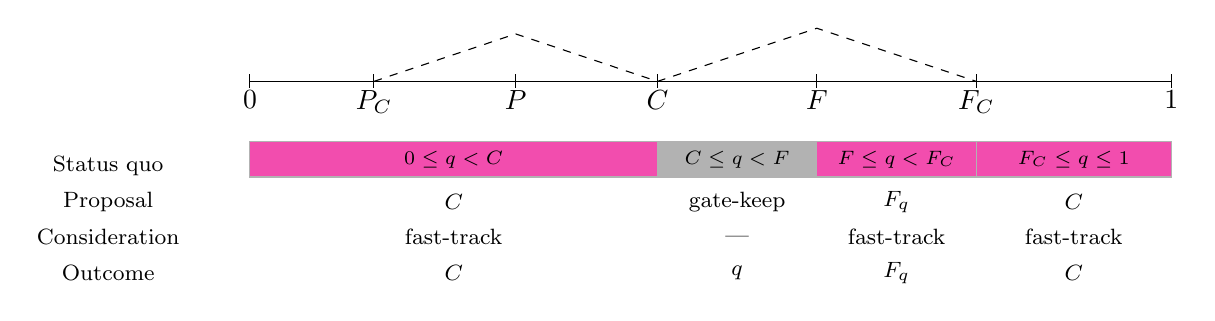
\begin{tikzpicture}[scale=.9]
          \draw (0,0) -- (13,0);
          \draw[dashed] (1.75,0) -- (3.75,0.67) -- (5.75,0);
          \draw[dashed] (5.75,0) -- (8,.75) -- (10.25,0);
          \draw (0,0.1) -- (0,-0.1) node[below=-0.1] {$0$}
          (1.75,0.1) -- (1.75,-0.1) node[below=-0.1] {$P_C$}
          (3.75,0.1) -- (3.75,-0.1) node[below=-0.1] {$P$}
          (5.75,0.1) -- (5.75,-0.1) node[below=-0.1] {$C$}
          (8,0.1) -- (8,-0.1) node[below=-0.1] {$F$}
          (10.25,0.1) -- (10.25,-0.1) node[below=-0.1] {$F_C$}
          (13,0.1) -- (13,-0.1) node[below=-0.1] {$1$};
          \node at (-2,-2.7) {\footnotesize{Outcome}};
          \node at (-2,-2.2) {\footnotesize{Consideration}};
          \node at (-2,-1.7)  {\footnotesize{Proposal}};
          \node at (-2,-1.2)  {\footnotesize{Status quo}};
          \node at (2.875,-2.7)   {\footnotesize{$C$}};          % Outcome      
          \node at (2.875,-2.2) {\footnotesize{fast-track}};         % Consideration
          \node at (2.875,-1.7)   {\footnotesize{$C$}};          % Proposal     
          \node at (6.875,-2.7)   {\footnotesize{$q$}};        % Outcome      
          \node at (6.875,-2.2) {\footnotesize{---}};            % Consideration
          \node at (6.875,-1.7)   {\footnotesize{gate-keep}};     % Proposal     
          \node at (9.125,-2.7)   {\footnotesize{$F_q$}};        % Outcome      
          \node at (9.125,-2.2) {\footnotesize{fast-track}};         % Consideration
          \node at (9.125,-1.7)   {\footnotesize{$F_q$}};        % Proposal     
          \node at (11.625,-2.7)   {\footnotesize{$C$}};          % Outcome      
          \node at (11.625,-2.2) {\footnotesize{fast-track}};         % Consideration
          \node at (11.625,-1.7)   {\footnotesize{$C$}};          % Proposal     
          \filldraw[fill=magenta!70,draw=black!30]   (0,-1.35) rectangle node {\scriptsize{$0 \leq q < C$}} (5.75,-0.85);
          \filldraw[fill=black!30,draw=black!30]  (5.75,-1.35) rectangle node {\scriptsize{$C \leq q < F$}} (8,-0.85);
          \filldraw[fill=magenta!70,draw=black!30]  (8,-1.35) rectangle node {\scriptsize{$F \leq q < F_C$}} (10.25,-0.85);
          \filldraw[fill=magenta!70,draw=black!30]  (10.25,-1.35) rectangle node {\scriptsize{$F_C \leq q \leq 1$}} (13,-0.85);
        \end{tikzpicture} \\ \\

        \textbf{II. Moderate president profile:} $C \leq P \leq F$ \\ 
        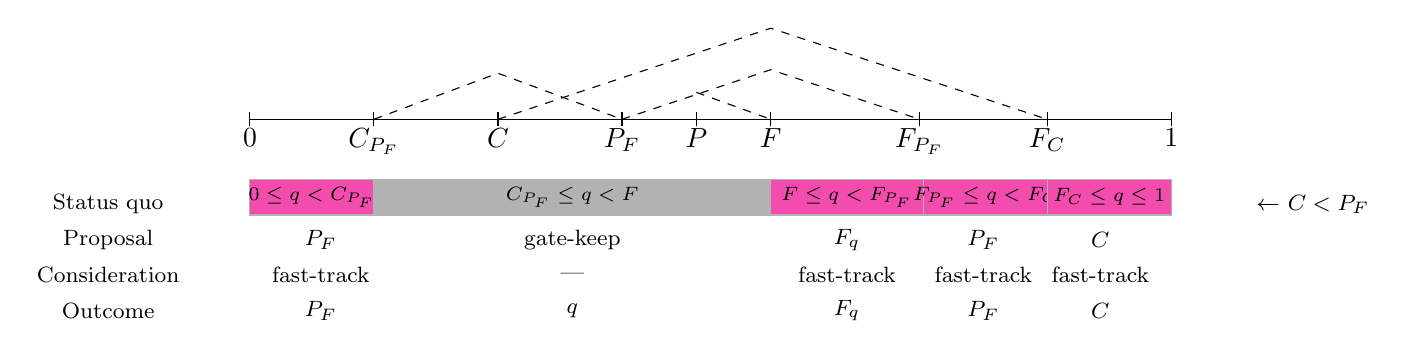
\begin{tikzpicture}[scale=.9]
          \draw (0,0) -- (13,0);
          \draw[dashed] (1.75,0) -- (3.5,0.65) -- (5.25,0);
          \draw[dashed] (3.5,0) -- (7.35,1.285) -- (11.25,0);
          \draw[dashed] (5.25,0) -- (7.35,.7) -- (9.45,0);
          \draw[dashed] (6.3,0.38) -- (7.35,0);
          \draw (0,0.1) -- (0,-0.1) node[below=-0.1] {$0$}
          (1.75,0.1) -- (1.75,-0.1) node[below=-0.1] {$C_{P_F}$}
          (3.5,0.1) -- (3.5,-0.1) node[below=-0.1] {$C$}
          (5.25,0.1) -- (5.25,-0.1) node[below=-0.1] {$P_F$}
          (6.3,0.1) -- (6.3,-0.1) node[below=-0.1] {$P$}
          (7.35,0.1) -- (7.35,-0.1) node[below=-0.1] {$F$}
          (9.45,0.1) -- (9.45,-0.1) node[below=-0.1] {$F_{P_F}$}
          (11.25,0.1) -- (11.25,-0.1) node[below=-0.1] {$F_C$}
          (13,0.1) -- (13,-0.1) node[below=-0.1] {$1$};
          \node at (-2,-2.7) {\footnotesize{Outcome}};
          \node at (-2,-2.2) {\footnotesize{Consideration}};
          \node at (-2,-1.7)  {\footnotesize{Proposal}};
          \node at (-2,-1.2)  {\footnotesize{Status quo}};
          \node at (15,-1.2)  {\footnotesize{$\leftarrow$ $C<P_F$}};
          \node at (1,-2.7)   {\footnotesize{$P_F$}};           % Outcome      
          \node at (1,-2.2) {\footnotesize{fast-track}};            % Consideration
          \node at (1,-1.7)   {\footnotesize{$P_F$}};           % Proposal     
          \node at (4.55,-2.7)   {\footnotesize{$q$}};           % Outcome      
          \node at (4.55,-2.2) {\footnotesize{---}};               % Consideration
          \node at (4.55,-1.7)   {\footnotesize{gate-keep}};        % Proposal     
          \node at (8.425,-2.7)   {\footnotesize{$F_q$}};           % Outcome      
          \node at (8.425,-2.2) {\footnotesize{fast-track}};            % Consideration
          \node at (8.425,-1.7)   {\footnotesize{$F_q$}};           % Proposal     
          \node at (10.35,-2.7)   {\footnotesize{$P_F$}};           % Outcome      
          \node at (10.35,-2.2) {\footnotesize{fast-track}};            % Consideration
          \node at (10.35,-1.7)   {\footnotesize{$P_F$}};           % Proposal     
          \node at (12,-2.7)   {\footnotesize{$C$}};             % Outcome      
          \node at (12,-2.2) {\footnotesize{fast-track}};            % Consideration
          \node at (12,-1.7)   {\footnotesize{$C$}};             % Proposal     
          \filldraw[fill=magenta!70,draw=black!30]   (0,-1.35) rectangle node {\scriptsize{$0 \leq q < C_{P_F}$}} (1.75,-0.85);
          \filldraw[fill=black!30,draw=black!30]  (1.75,-1.35) rectangle node {\scriptsize{$C_{P_F} \leq q < F$}} (7.35,-0.85);
          \filldraw[fill=magenta!70,draw=black!30]  (7.35,-1.35) rectangle node {\scriptsize{$F \leq q < F_{P_F}$}} (9.5,-0.85);
          \filldraw[fill=magenta!70,draw=black!30]  (9.5,-1.35) rectangle node {\scriptsize{$F_{P_F} \leq q < F_C$}} (11.25,-0.85);
          \filldraw[fill=magenta!70,draw=black!30]  (11.25,-1.35) rectangle node {\scriptsize{$F_C \leq q \leq 1$}} (13,-0.85);
        \end{tikzpicture} \\ \\

        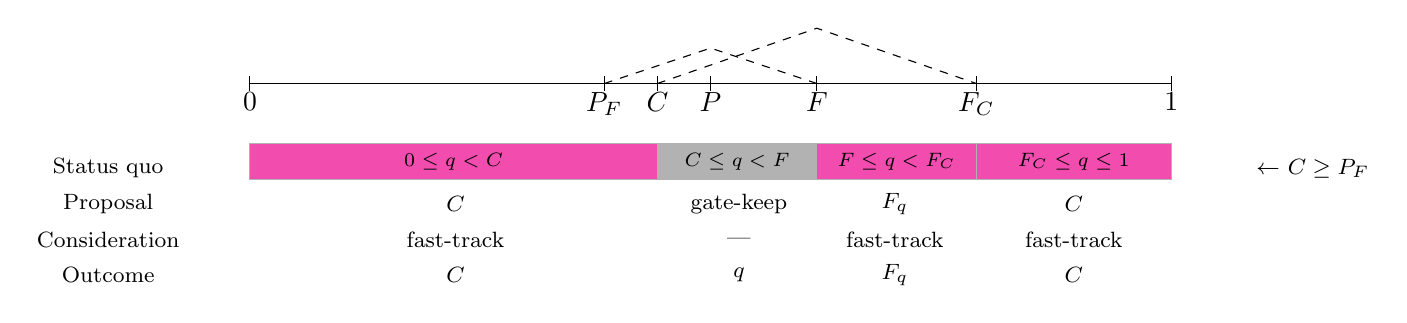
\begin{tikzpicture}[scale=.9]
          \draw (0,0) -- (13,0);
          \draw[dashed] (5,0) -- (6.5,0.5) -- (8,0);
          \draw[dashed] (5.75,0) -- (8,.78) -- (10.25,0);
          \draw (0,0.1) -- (0,-0.1) node[below=-0.1] {$0$}
          (5,0.1) -- (5,-0.1) node[below=-0.1] {$P_F$}
          (5.75,0.1) -- (5.75,-0.1) node[below=-0.1] {$C$}
          (6.5,0.1) -- (6.5,-0.1) node[below=-0.1] {$P$}
          (8,0.1) -- (8,-0.1) node[below=-0.1] {$F$}
          (10.25,0.1) -- (10.25,-0.1) node[below=-0.1] {$F_C$}
          (13,0.1) -- (13,-0.1) node[below=-0.1] {$1$};
          \node at (-2,-2.7) {\footnotesize{Outcome}};
          \node at (-2,-2.2) {\footnotesize{Consideration}};
          \node at (-2,-1.7)  {\footnotesize{Proposal}};
          \node at (-2,-1.2)  {\footnotesize{Status quo}};
          \node at (15,-1.2)  {\footnotesize{$\leftarrow$ $C \geq P_F$}};
          \node at (2.9,-2.7)   {\footnotesize{$C$}};        % Outcome      
          \node at (2.9,-2.2) {\footnotesize{fast-track}};       % Consideration
          \node at (2.9,-1.7)   {\footnotesize{$C$}};        % Proposal     
          \node at (6.9,-2.7)   {\footnotesize{$q$}};      % Outcome      
          \node at (6.9,-2.2) {\footnotesize{---}};          % Consideration
          \node at (6.9,-1.7)   {\footnotesize{gate-keep}};   % Proposal     
          \node at (9.1,-2.7)   {\footnotesize{$F_q$}};      % Outcome      
          \node at (9.1,-2.2) {\footnotesize{fast-track}};       % Consideration
          \node at (9.1,-1.7)   {\footnotesize{$F_q$}};      % Proposal     
          \node at (11.625,-2.7)   {\footnotesize{$C$}};         % Outcome      
          \node at (11.626,-2.2) {\footnotesize{fast-track}};        % Consideration
          \node at (11.625,-1.7)   {\footnotesize{$C$}};         % Proposal     
          \filldraw[fill=magenta!70,draw=black!30]   (0,-1.35) rectangle node {\scriptsize{$0 \leq q < C$}} (5.75,-0.85);
          \filldraw[fill=black!30,draw=black!30]  (5.75,-1.35) rectangle node {\scriptsize{$C \leq q < F$}} (8,-0.85);
          \filldraw[fill=magenta!70,draw=black!30]  (8,-1.35) rectangle node {\scriptsize{$F \leq q < F_C$}} (10.25,-0.85);
          \filldraw[fill=magenta!70,draw=black!30]  (10.25,-1.35) rectangle node {\scriptsize{$F_C \leq q \leq 1$}} (13,-0.85);
        \end{tikzpicture} \\ \\

        \textbf{III. Moderate floor profile:} $C <  F <  P$ \\ 
        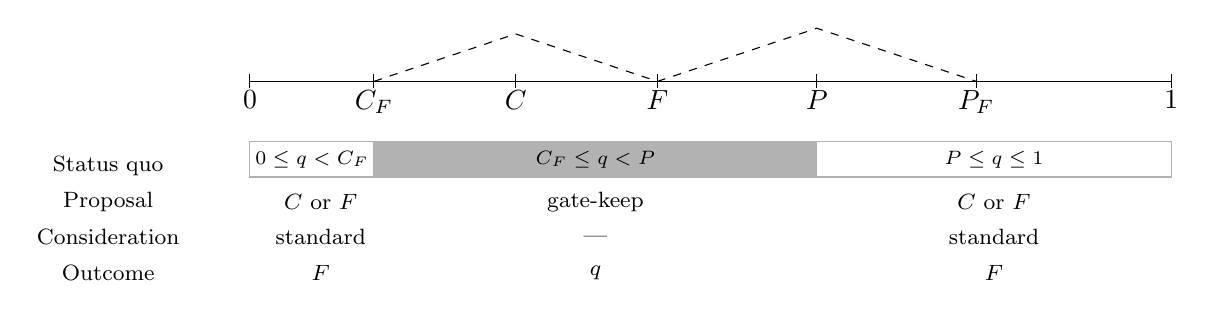
\begin{tikzpicture}[scale=.9]
          \draw (0,0) -- (13,0);
          \draw[dashed] (1.75,0) -- (3.75,0.67) -- (5.75,0);
          \draw[dashed] (5.75,0) -- (8,.75) -- (10.25,0);
          \draw (0,0.1) -- (0,-0.1) node[below=-0.1] {$0$}
          (1.75,0.1) -- (1.75,-0.1) node[below=-0.1] {$C_F$}
          (3.75,0.1) -- (3.75,-0.1) node[below=-0.1] {$C$}
          (5.75,0.1) -- (5.75,-0.1) node[below=-0.1] {$F$}
          (8,0.1) -- (8,-0.1) node[below=-0.1] {$P$}
          (10.25,0.1) -- (10.25,-0.1) node[below=-0.1] {$P_F$}
          (13,0.1) -- (13,-0.1) node[below=-0.1] {$1$};
          \node at (-2,-2.7) {\footnotesize{Outcome}};
          \node at (-2,-2.2) {\footnotesize{Consideration}};
          \node at (-2,-1.7)  {\footnotesize{Proposal}};
          \node at (-2,-1.2)  {\footnotesize{Status quo}};
          \node at (1,-2.7)   {\footnotesize{$F$}};              % Outcome      
          \node at (1,-2.2) {\footnotesize{standard}};           % Consideration
          \node at (1,-1.7)   {\footnotesize{$C$ or $F$}};              % Proposal     
          \node at (4.875,-2.7)   {\footnotesize{$q$}};         % Outcome      
          \node at (4.875,-2.2) {\footnotesize{---}};             % Consideration
          \node at (4.875,-1.7)   {\footnotesize{gate-keep}};      % Proposal     
          \node at (10.5,-2.7)   {\footnotesize{$F$}};          % Outcome      
          \node at (10.5,-2.2) {\footnotesize{standard}};       % Consideration
          \node at (10.5,-1.7)   {\footnotesize{$C$ or $F$}};   % Proposal     
          \filldraw[fill=black!0,draw=black!30]   (0,-1.35) rectangle node {\scriptsize{$0 \leq q < C_F$}} (1.75,-0.85);
          \filldraw[fill=black!30,draw=black!30]  (1.75,-1.35) rectangle node {\scriptsize{$C_F \leq q < P$}} (8,-0.85);
          \filldraw[fill=black!0,draw=black!30]  (8,-1.35) rectangle node {\scriptsize{$P \leq q \leq 1$}} (13,-0.85);
        \end{tikzpicture} \\ \\

      \end{tabular}
    }
\end{figure}

Under what conditions will presidents fast-track legislation? And what conditions will make them willing to allow for open rules? To answer, and by doing so derive empirical implications, we extend the bargaining logic across preference profiles. A preference profile is an ordering of players' ideal points in space. Three profiles are portrayed in Figure \ref{F:predictions}, distinguishing which player is moderate relative to the others: the committee ($P<C<F$), the president ($C \leq P \leq F$), and the floor ($C<F<P$); the other mutually-exclusive and exhaustive profiles are mirror-images. The example from Figure 2 belongs in the moderate committee profile I, but we now treat the status quo as a variable $q \in [0,1]$---the example's is in $0 \leq q < C$. The figure traces how changes in $q$ affect three measures of interest: the proposal, the consideration regime, and the game's outcome. Each discrete zone (the pink, gray, or white rectangles) keeps status quos with unchanging equilibrium components together.

The first thing to notice is that fast-track occurs only when the president and committee ideal points lie on the same side of the floor median (i.e., a profile other than the moderate floor is a necessary condition for the fast track). We assume that committees are unitary actors where chairs are dictators; and that players from the same party have closer ideal points than players from different parties.\footnote{House rules in Chile (see n.~\ref{fn:comm-chains}) and party discipline \citep{aleman.saiegh.coalUnityChile.2007,carey.2002} support these assumption in the Chilean case. Derivation involves the more technical auxiliary assumption of a stochastic status quo whose probability distibution has support in $[0,1]$---i.e., $q$ occurs in any range of the policy space with non-zero probability. Dropping it creates discontinuities in prediction, which complicate exposition. See \citet[, 38]{cox.mccubbins.2005} for an elaboration.} Thus, the results show that when the committee chair and the president have close preferences relative to the floor---that is, when they lie on the same side of $F$---the bill coming out from committee will be considered under urgent procedures. 

In other words, when the president and the committee chair belong to the same party, they will be able to negotiate a bill that is acceptable to both of them. Under such circumstances, the president will have an incentive to declare the bill urgent so she can prevent floor amendmets that would otherwise move the bill further away. The president does not utilize the urgency to accelerate bill approval, but instead uses it to protect the bill from unwanted amendments on the floor. In this sense, the president takes on the role of the Rules Committee, deciding whether the bill will reach the floor under closed or open rules. Our first hypothesis reflects the conditions under which the president will use her urgency authority.

\begin{description}
  \item [Hypothesis 1:] Presidents are more likely to fast-track bills when the committee chair with jurisdiction over the bill  belongs to the president's party than otherwise.
\end{description}

The hypothesis is not independent of the location of floor preferences with respect to the president, and clearly, when floor preferences are closer to the president than the preferences of the committee chair, the necessity to fast track bills declines. To see this, hold the distance separating $P$ and $F$ constant while shrinking the distance between $C$ and $P$ and see what happens in each profile. Magenta rectangles become more prominent relative to gray ones in I and II (the probability of the fast-track goes up) but not in III (where the fast-track probability remains unchanged). 

The other important result refers to the conditions under which the president will decide not to use her urgency authority.  Figure \ref{F:predictions} shows that standard bill consideration (white rectangles) occurs under the moderate floor profile only, when committee and president are on either side of the floor median. This means that when the preferences of the committee and the president are farther apart---i.e., they belong to different parties---the president will not get in the way of open rule consideration of bills. By allowing amendments, which bring policy towards $F$, the president will be able to move the bill closer to her ideal point. Thus, if a committee chair belongs to an opposition party, the president has the power to influence bills by allowing the regular procedure (open rule) to operate, that is, by desisting from using her urgency authority. Thus, our second hypothesis refers to the conditions under which the president will refrain from fast-tracking bills.\footnote{Empirical implications about other measures of interest, such as gatekeeping and expected bargaining outcomes, also follow from models in the spatial family. We did not systematize data from bill histories to test these implications, so we do not discuss them here.} 

\begin{description}
  \item [Hypothesis 2:] Presidents are more likely to allow open rule consideration of bills when the committee chair with jurisdiction over the bill belongs to a party that is not in the president's coalition than otherwise.
\end{description}

We replace ``party'' with ``coalition'' as an alternative measure of preferences in the test. Chilean politics since 1990 has operated under the coalition logic. Two main coalitions, one from the center-right and the other from the center-left, work cohesively in government and in the opposition. Coalition discipline is well-documented \citep{carey.2002,aleman.saiegh.coalUnityChile.2007}. 


\section*{Data and Analysis}

We collected original data to test the hypothesis, compiling bill histories of every draft law that the executive introduced in Congress between 1998 and 2014:\footnote{We scraped the \emph{C\'amara de Diputados'} web page (\url{www.camara.cl}) in November 2014 to retrieve the record (\emph{bolet\'in}) of every proposal made between 11 March 1998 and 10 March 2014, inclusive. Data and commented code for replication accompany the online appendix. We conducted data analysis with a multiplicity of \texttt{R}'s libraries.} when each was introduced, in which chamber of the bicameral Congress, the issue it deals with, the status at the time of consultation, and so forth. We also gathered information on the chronological detail of the bill's legislative process in the House: committee referrals and reports, floor discussion and voting, when it was sent to the Senate, and more. Of direct relevance, we coded all bills marked urgent in the \emph{C\'amara de Diputados}. Earlier years antedate Internet publication and were dropped, as data completeness in the primary source remains to be verified. The period selected fully covers two Senates, four \emph{C\'amaras}, and three presidencies (plus the last two years of an earlier presidency).

\begin{table}
\centering
\caption{Proposals, legislation, and fast-track authority}\label{T:billDescriptives}
\begin{tabular}{llrr}
\multicolumn{4}{c}{\textbf{Part A. Executive bills}} \\
   & \multicolumn{2}{l}{Bills}                           &   frequency  \\ \hline
I  & \multicolumn{2}{l}{introduced}                      &       1,467  \\ \hdashline
II & \multicolumn{2}{l}{passed}                          &       1,059  \\
   & \multicolumn{2}{l}{as \% of introduced}             &   \emph{72}  \\ \hdashline
III& \multicolumn{2}{l}{fast-tracked}                    &         540  \\
   & \multicolumn{2}{l}{as \% of introduced}             &   \emph{37}  \\ \hdashline
IV & \multicolumn{2}{l}{fast-tracked \& passed}          &         415  \\
   & \multicolumn{2}{l}{as \% of fast-tracked}           &   \emph{77}  \\ \hline
\\
\multicolumn{4}{c}{\textbf{Part B. Urgent bills by presidency}} \\
\multicolumn{2}{l}{President and period}    & $N$ bills & \% fast-tracked \\ \hline
\multicolumn{2}{l}{Frei 1998--2000$^\dagger$} & 128       &  \emph{38} \\
\multicolumn{2}{l}{Lagos 2000--2006}        & 544       &  \emph{25} \\
\multicolumn{2}{l}{Bachelet 2006--2010}     & 392       &  \emph{39} \\
\multicolumn{2}{l}{Pi\~nera 2010--2014}       & 403       &  \emph{50} \\ \hdashline
\multicolumn{2}{l}{All 1998--2014}          & 1,467     &  \emph{37} \\
\hline
\multicolumn{4}{r}{\footnotesize{$^\dagger$ Last third of the six-year term in the analysis only.}} \\
\end{tabular}
\end{table}

Table \ref{T:billDescriptives} offers a general summary of bill introductions, passages, and fast-track incidences. The executive sent 1,467 bills to Congress between 1998 and 2014, on average ninety-one yearly. (Members of Congress proposed 79 percent of all bills, not analyzed.) More than one thousand proposals became law during the period, putting the executive's success rate at 72 percent---high by Latin American standards \citep{morgenstern.nacif.2002}. And 540 bills were on the fast-track during lower chamber consideration, 37 percent of all bills introduced. And 77 percent of those became law, so about 40 percent of bills that became law did it under restrictive procedures. 

The variance in urgency incidence across administrations, reported in part B, is considerable. But differences in urgency authority usage do not seem related with specifics traits of the president. For instance, one could argue that presidents with previous legislative experience might be less inclined to interfere with Congressional priorities. Frei (with previous legislative experience) and Bachelet (without) were about on average, Lagos (with experience) quite below, and Pi\~nera (without) quite above.

\subsection*{Fast-Track predictors}

Multivariate analysis of the data is revealing. The unit of analysis is individual executive proposals: the dependent variable \emph{Fast-tracked Bill} equals 1 for proposals marked with `supreme urgency' while in the C\'amara, 0 otherwise. Our main independent variable accounts for preference coincidence between the president and the reporting committee. We include controls for bill features, for timing, and for the strategic environment. Formal variable definitions and descriptive statistics appear in the online appendix.

With respect to our main independent variable, which accounts for preferences, we include \emph{Co-partisan Chair} and \emph{Coalition Chair}, which seek to identify committee chairs' preference location vis-\`a-vis the president, and \emph{Multiple Referrals}, which identifies bills referred to multiple committees. \emph{Co-partisan Chair} equals 1 if the bill was referred to a standing committee presided by a member of the president's party, and equals 0 otherwise; \emph{Coalition Chair} equals 1 for bills referred to committees chaired by members of any party in the presidential coalition, 0 otherwise. These are two different ways in which we measure our key explanatory variable, spatial proximity between the chief executive and the reporting committee, and we expect each to associate positively with the dependent variable. Part A of Table \ref{T:chairsSeats} shows that the number of standing committee chairs in hands of the president's party varied in the period, from a high of 53 percent in the 1998--2002 legislature to a low of 17 percent in 2006--10. And the opposition chaired no standing committee in 2006--10, but up to 24 and 27 percent in 2002--06 and 2010--14, respectively.\footnote{\emph{Largesse} towards opposition parties was probably aimed at beefing up the president's legislative support. Unlike the Senate, the coalition remained in control of the C\'amara throughout the period. But, by requiring 67, 60, and 57 percent votes of each chamber, respectively, constitutional reform, constitution-interpreting legislation, and organic laws therefore always required support across the aisle.}

\begin{table}
\centering
\caption{The president's status in Congress and its committees. Percent chairs/seats by party. The president's coalition in 1998--2010 was Concertaci\'on; it was Alianza afterwards. Regional includes major-party splinters (from Christian Democrats and Uni\'on Dem\'ocrata Independiente). President's status in the Senate slightly and briefly oscillated above and below majority due to vacant seats. Source: prepared with information from \protect\url{www.camara.cl}.}\label{T:chairsSeats}
\begin{tabular}{lrrrr}
                      & 1998--2002 & 2002--06 & 2006--10 & 2010--14 \\ \hline
\mc{5}{c}{\textbf{~~Part A. Committee chairs, C\'amara}} \\
President's party     &  \emph{53} & \emph{35}  & \emph{17}  & \emph{23}   \\
Other coalition party &  \emph{41} & \emph{41}  & \emph{83}  & \emph{50}   \\
Opposition            &   \emph{6} & \emph{24}  &            & \emph{27}   \\ \hdashline
Total                 & \emph{100} & \emph{100} & \emph{100} & \emph{100}  \\ 
$N$ standing committees&  17        &  17      &  18      & 22      \\ [1.8ex] \hline 
\mc{5}{c}{\textbf{~~Part B. Seats, C\'amara}} \\ 
President's coalition & \emph{58}     & \emph{53}  & \emph{51}   & \emph{50}   \\
Opposition            & \emph{42}     & \emph{48}  & \emph{47}   & \emph{48}   \\
Regional              &               &            & \emph{3}    & \emph{2}    \\ \hdashline
Total       & \emph{100}    & \emph{100} & \emph{100}  & \emph{100}  \\ [1.8ex] \hline
\mc{5}{c}{\textbf{~~Part C. Seats, Senate}} \\
President's coalition & \emph{50}            & \emph{50}       & \emph{55}   & \emph{45}       \\
Opposition            & \emph{50}            & \emph{50}       & \emph{45}   & \emph{55}       \\ \hdashline
Total                 & \emph{100}$^{\dagger}$ & \emph{100}      & \emph{100}  & \emph{100}      \\ \hline
\mc{5}{r}{\footnotesize{$^\dagger$vacant seats dropped}}
\end{tabular}
\end{table}

We also control for multiple referrals. Nearly one quarter (24 percent) of bills in the period were referred to more than one standing committee. The ``other committee'' count excludes the Finance Committee, with jurisdiction over any form of new spending (and discussed next---multiple referrals reach 32 percent when the Finance Committee is considered). Also excluded are special and bicameral committees. \emph{Multiple Referrals} should capture any effect of agenda control sharing among several committee chairs during the proposal's negotiation---reflecting the need to rein on unruly chairs through a friendlier committee. A single co-partisan or coalition chair among multiple referees suffices for the indicator previously discussed to equal 1. 

The variable intended to capture bill-specific features is \emph{Hacienda Referral}, which equals 1 for bills referred to the powerful Finance Committee with special status in the Chilean Congress, 0 otherwise. Unlike other standing committees, the Finance Committee has jurisdiction over \emph{every} bill authorizing spending in any domain. Moreover, the unanimous exception rule discussed earlier is inapplicable to \emph{Hacienda} bills, which must be reported prior to floor consideration.\footnote{\emph{Ley Org\'anica del Congreso} arts.\ 17 and 21.} Committee members, working in tandem with the Finance Ministry, may or may not appropriate funds from the budget in their report \citep{aleman.navia.UrgChi.2009}. Not unlike the Appropriations and Rules committees in the U.S.\ House, \emph{Hacienda} has the status of a control committee, a key asset for agenda power \citep{kiewiet.mccubbins.1991}. \emph{Hacienda} referral therefore controls for a subset of generally important proposals, and we expect it to associate positively with urgency authority.

Three controls account for the strategic environment. \emph{Presidential Approval} is the net general population presidential approval rate at bill initiation (i.e., the percentage of respondents who approve of the president's job minus the percentage who disapprove). We have no a priori expectation here. If presidents with better public opinion standing are also more successful in the legislative arena \citep{bond.fleisher.1990,aleman.navia.UrgChi.2009}, they might also need restrictive rules less often, and reliance on the fast-track might therefore drop (in some issue areas, at least).\footnote{We estimate the models using subsets of bills by issue area in the online appendix. Smaller numbers of bills tend to hamper statistical significance, but the results are in line with those reported.} The contrary might hold if popular presidents were more successful in obtaining more likeable reports from the average committee chair, that would then require protection against floor amendments. \emph{Introduced in Senate} equals 1 for bills sent to the Upper Chamber, 0 otherwise. By virtue of being smaller, enjoying longer terms, and not being firmly under the president's coalition control during most of the period, bills sent to the Senate might present systematic differences in fast-track usage. And \emph{Senate Majority} equals 1 if the president's coalition controlled half or more of Upper Chamber seats when the bill was initiated, 0 otherwise.\footnote{Parties in the presidential and opposition coalitions were tied throughout most of the 1998--2006 Senate (majority briefly oscillating back and forth in the first years due to member indictments, impeachments, and deaths in both coalitions). Ties are coded as \emph{Senate Majority} = 1.} Other things equal, presidents with sufficient partisan legislative resources in both chambers will find it easier to push proposals through Congress, and might be less inclined to use the fast-track prerogative to successfully navigate log-rolls through the plenary session.

The group of variables accounting for time-related effects control for different aspects of the congressional cycle. \emph{Year Remaining} (and its squared value to capture non-linearity, if any) measures the percentage of the legislative year remaining at bill initiation. Chilean legislative years start after the (meridional) summer break. So the variable adopts value 100 for proposals introduced on March 1 (the first day of the legislative year), and value 0 for proposals introduced the last day of February. It should control for stationarity in the data (the online appendix elaborates the temporal dimension in the use of urgencies). And \emph{Relax Deadline} equals 1 for bills initiated in July 2010 or later, 0 otherwise. Congress doubled deadlines to consider and vote urgent bills five months into the 2010--14 legislature (see online appendix). Any systematic shift in urgency usage attributable to this reform should be reflected in this coefficient. 

\subsection*{Model Specification and Results}

Given that we pool observations from four elected legislatures, with important differences in the types and the volume of proposals considered \citep{aleman.navia.UrgChi.2009}, heterogeneity might interfere. We fit two additional model specifications for robustness verification. One includes fixed legislature effects---i.e., three dummies for bills initiated in the 2002--06, 2006--10, and 2010--14 periods, respectively; the excluded 1998--2002 dummy is the baseline. Another adds further flexibility by also estimating separate errors for bills initiated in each legislature \citep[a so-called mixed effects model,][, 262, 302]{gelman.hill.2007}. We rely on a generalized linear model for mixed effects estimation, and logit for the rest. We normalized continuous variables \emph{Presidential Approval} and \emph{Year Remaining} to speed the GLM's convergence.\footnote{As suggested in \url{http://stackoverflow.com/questions/23478792/warning-messages-when-trying-to-run-glmer-in-r} and \url{https://rstudio-pubs-static.s3.amazonaws.com/33653_57fc7b8e5d484c909b615d8633c01d51.html}. Normalization re-scales and centers the measures in order to improve parameter identification.} Normalized measures were used throughout for model comparability.

% Table created by stargazer v.5.2 by Marek Hlavac, Harvard University. E-mail: hlavac at fas.harvard.edu
% Requires LaTeX packages: dcolumn 
\begin{table}
  \centering 
  \caption{Executive bill fast-track predictors. Standard errors in parentheses. Model 3 includes fixed Legislatura effects (not reported). Model 4 estimates separate error terms by Legislatura. Method of estimation: model 4 with generalized linear model, others with logit \citep[fitted with \texttt{R} base's \texttt{glm} and library \texttt{lme4},][]{lme4.2015}.}\label{t:urgenLogit}
  \begin{tabular}{@{\extracolsep{0pt}}lD{.}{.}{-3} D{.}{.}{-3} D{.}{.}{-3} D{.}{.}{-3} } 
    \hline \\[-1.8ex] 
    & \multicolumn{4}{c}{DV: Bill on fast-track (1) or not (0)} \\ 
    \\[-1.8ex] & \multicolumn{1}{c}{(1)} & \multicolumn{1}{c}{(2)} & \multicolumn{1}{c}{(3)} & \multicolumn{1}{c}{(4)}\\ 
    \\ [-1.8ex] 
    \hline \\[-1.8ex] 
    \emph{Co-partisan}     &  .289^{**}   &  &  &                                   \\
    \emph{Chair}           & (.024)      &  &  &                                   \\ [.75ex]
    \emph{Coalition}       &             & .825^{***}   & .874^{***}    & .847^{***}   \\
    \emph{Chair}           &             & (.005)      & (<.001)     & (<.001)     \\ [.75ex]
    \emph{Multiple}        &  .772^{***}  &  .795^{***}  &  .808^{***}   &  .809^{***}   \\
    \emph{Referrals}       & (<.001)     & (<.001)     & (<.001)     & (.004)      \\ [.75ex]
    \emph{Hacienda}        & 1.002^{***}  & .940^{***}   & .917^{***}    & .923^{***}    \\
    \emph{Referral}        & (<.001)     & (<.001)     & (<.001)     & (<.001)     \\ [.75ex]
    \emph{Pres.}           &  -.078      &  -.096      &  .029       & -.044       \\
    \emph{Approval}        & (.286)      & (.187)      & (.710)      & (.567)      \\ [.75ex]
    \emph{Introduced}      &  -.716^{***} &  -.698^{***}  &  -.744^{***} &  -.730^{***}  \\
    \emph{in Senate}       & (<.001)     & (<.001)     & (<.001)      & (<.001)    \\ [.75ex]
    \emph{Senate}          &  -.251      &  -.319      &             &             \\
    \emph{Majority}        & (.214)      & (.110)      &             &             \\ [.75ex]
    \emph{Year}            &  .072       &  .065       &  .053        &  .053      \\
    \emph{Remaining}       & (.223)      & (.268)      & (.370)       & (.368)     \\ [.75ex]
    \emph{(Year}           &  -.224^{***} &  -.238^{***}  &  -.255^{***}  &  -.251^{***} \\
    \emph{Remaining)$^2$}  & (<.001)     & (<.001)      & (<.001)     & (<.001)    \\ [.75ex]
    \emph{Relax}           &  .479^{*}    &  .394       &              &            \\
    \emph{Deadline}        & (.057)      & (.104)      &              &            \\ [.75ex]
    %% \emph{2002-06 Leg.} &  &  &  -.203 &                                        \\
    %%                     &  &  & (.298) &                                        \\ [.75ex]
    %% \emph{2006-10 Leg.} &  &  &  .302^{*} &                                     \\
    %%                     &  &  & (.097) &                                        \\ [.75ex]
    %% \emph{2010-14 Leg.} &  &  & 1.200^{***} &                                   \\
    %%                     &  &  & (<.001) &                                       \\ [.75ex]
    Intercept              &  -1.046^{***} & -1.589^{***} & -1.933^{***} & -1.719^{***}  \\
                           & (<.001)      & (<.001)     & (<.001)    & (<.001)     \\ [.75ex]
    \hline \\[-1.8ex] 
    Effects & \multicolumn{1}{c}{none} & \multicolumn{1}{c}{none} & \multicolumn{1}{c}{fixed} & \multicolumn{1}{c}{mixed} \\ 
    Observations & \multicolumn{1}{c}{1,467} & \multicolumn{1}{c}{1,467} & \multicolumn{1}{c}{1,467} & \multicolumn{1}{c}{1,467} \\ 
    Log$L$ & \multicolumn{1}{c}{$-864$} & \multicolumn{1}{c}{$-862$} & \multicolumn{1}{c}{$-852$} & \multicolumn{1}{c}{$-859$} \\ 
    \% correct & \multicolumn{1}{c}{67} & \multicolumn{1}{c}{68} & \multicolumn{1}{c}{68} & \multicolumn{1}{c}{68} \\ 
%%Akaike Inf. Crit. & \multicolumn{1}{c}{1,748.896} & \multicolumn{1}{c}{1,740.400} & \multicolumn{1}{c}{1,719.057} & \multicolumn{1}{c}{1,731.050} \\ 
%%Bayesian Inf. Crit. &  &  &  & \multicolumn{1}{c}{1,778.632} \\ 
    \\ [-1.8ex] 
    \hline \\[-1.8ex] 
    & \multicolumn{4}{r}{\footnotesize $^{*}$p$<$.1; $^{**}$p$<$.05; $^{***}$p$<$.01 (p-values in parentheses)} \\ 
  \end{tabular} 
\end{table} 

Table \ref{t:urgenLogit} reports results.\footnote{The regression model performs satisfactorily. A likelihood-ratio test of overall fit rejects the hypothesis, at below the .001 level, that an intercept-only fit is as good as our models. Predictors across model specifications correctly classify 67--68 percent of the observations.} We find support for our main hypothesis. In line with expectations, both variables measuring the proximity of committee chairs to the president increase the probability of fast-track. \emph{Co-partisan Chair} has a positive coefficient in model 1, as hypothesized, and the effect achieves conventional statistical significance (parentheses in the table report p-values). The evidence is much stronger for the variable's other specification: the coefficient for \emph{Coalition Chair} in models 2--4 is also positive, triples its size, and achieves p-values at .005 or below. In other words, if a bill is referred to a committee where the president finds support (either because the chair belongs to her party or to her coalition), the report is more likely to be fast-tracked for floor consideration. This matches previous scholarship, i.e., that the coalition is as good a predictor of presidential support in Congress---or better, in our case---as the party. The finding is robust across model specifications. In general, all model coefficients remain pretty much unchanged in size and significance when fixed and mixed effects are included on the right side (\emph{Senate Majority} and \emph{Relax Deadline} must be dropped due to colinearity with legislature dummies). 

%% > mar3
%%      factor     AME     SE       z      p   lower   upper
%%   dsameCoal  0.1734 0.0585  2.9651 0.0030  0.0588  0.2880
%%   dmultiRef  0.1603 0.0250  6.4003 0.0000  0.1112  0.2093
%%     drefHda  0.1817 0.0232  7.8483 0.0000  0.1363  0.2271
%%  netApprovR -0.0030 0.0153 -0.1976 0.8433 -0.0331  0.0270
%%      dinSen -0.1475 0.0335 -4.3981 0.0000 -0.2132 -0.0818
%%      legyrR  0.0173 0.0120  1.4463 0.1481 -0.0062  0.0408
%%     legyrR2 -0.0535 0.0127 -4.2213 0.0000 -0.0784 -0.0287
%%   legis2002 -0.0628 0.0374 -1.6802 0.0929 -0.1360  0.0105
%%   legis2006  0.0525 0.0370  1.4185 0.1561 -0.0200  0.1249
%%   legis2010  0.1813 0.0389  4.6590 0.0000  0.1050  0.2575

\begin{figure}
  \centering
    \caption{Average marginal effects from model 3. Dots report how the probability of an urgent bill changes in response to a unit change in each independent variable, all else at mean values; bars are 95-percent confidence intervals.}\label{F:avgMg}
    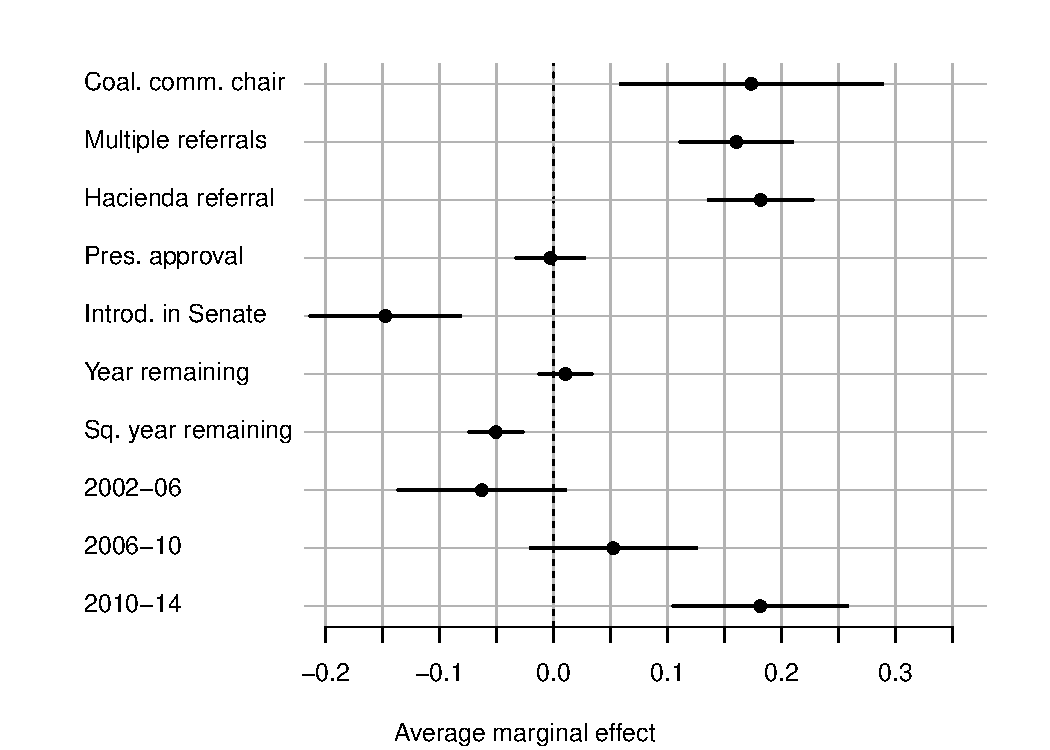
\includegraphics[width=.8\columnwidth]{../graphs/avgMgEffects.pdf}
\end{figure}

Figure \ref{F:avgMg} reports changes in the average predicted probability that a bill is fast-tracked associated with unit changes in model 3's explanatory variables (all other regressors at their mean value). This is a convenient way to gauge logit regression coefficients, by translating them into interpretable quantities. The report from a committee with a coalition chair experiences a 0.17 hike (0.06 standard error) in the likelihood of receiving a closed rule compared to a report by an opposition-chaired committee. The effect is as big as the average marginal effects of \emph{Hacienda Referral} (0.18), which capures mostly high-significance draft laws, and that of \emph{Multiple Referrals} (0.16), which we view as an indicator of issue complexity. We therefore find no statistical evidence to reject our Hypothesis 1. The results also confirm hypothesis 2, showing that a bill reported by a generally less friendly committe (chaired by the opposition), has a higher probability of receiving an open rule on the floor, thereby allowing the floor majority to bring back the bill to the median through floor amendments. Thus, presidents use open rules to control bills coming from preference distant committee chairs.

The substantial effects of \emph{Hacienda Referral} and \emph{Multiple Referrals} deserve comment. They suggest, first, that when spending gets in the way, restrictive rules are the norm in Chile. Recall that \emph{Multiple Referrals} exclude the Finance Committee, so there is an independent effect of bills with jurisdictional overlaps worth investigating further, and which must be associated, in part at least, to influencing the report through a friendlier committee.\footnote{We are grateful for this insight from an anonymous referee. According to \citet[][, 118]{sotoCongChile2015}, multiple-referees may act sequentially or in tandem, as decided by the C\'amara's presiding officer. When sequential, a divergent secondary committee's report is treated as an amendment to the primary committee's---an urgency overrides the secondary (and subsequent) report(s). We unfortunately lack information on this important aspect of multiple referrals.} Furthermore, note that the Finance Committee was always chaired by a coalition member but, with the exception of the 1998--2000 period, never by a co-partisan of the president. This may explain the milder effect of the partisan specification of our key variable in model 1. 

Another effect worth highlighting is \emph{Introd.\ in Senate}. Bills successfully passing the Upper Chamber first, where the opposition was systematically larger and at times in control, were much less likely to get urgent status (the average marginal effect is $-0.15$ and significant). This suggests that agreements and compromises reached in the Senate ignited less, not more, protection from floor amendments in the \emph{C\'amara's} plenary, most likely as a consequence of the greater preference divergence between the President and the opposition-led Senate. Analysis of inter-chamber negotiation and the reliance on urgency in the Upper Chamber are interesting venues for future research. 

\begin{figure}
  \centering
    \caption{Probability of fast-track bill consideration. Predictions are from from model 3 letting \emph{Year Remaining} vary in full range, with 95\% confidence bands. Other variables set at the following values: $\text{\emph{Multiple Referrals}}=0$, $\text{\emph{Hacienda Referral}}=0$, $\text{\emph{Introd.~in~Senate}}=0$, $\text{\emph{2006-10}}=1$, and $\text{\emph{Pres.~Approval}}=.33$ (Bachelet's mean).}\label{F:sims}
    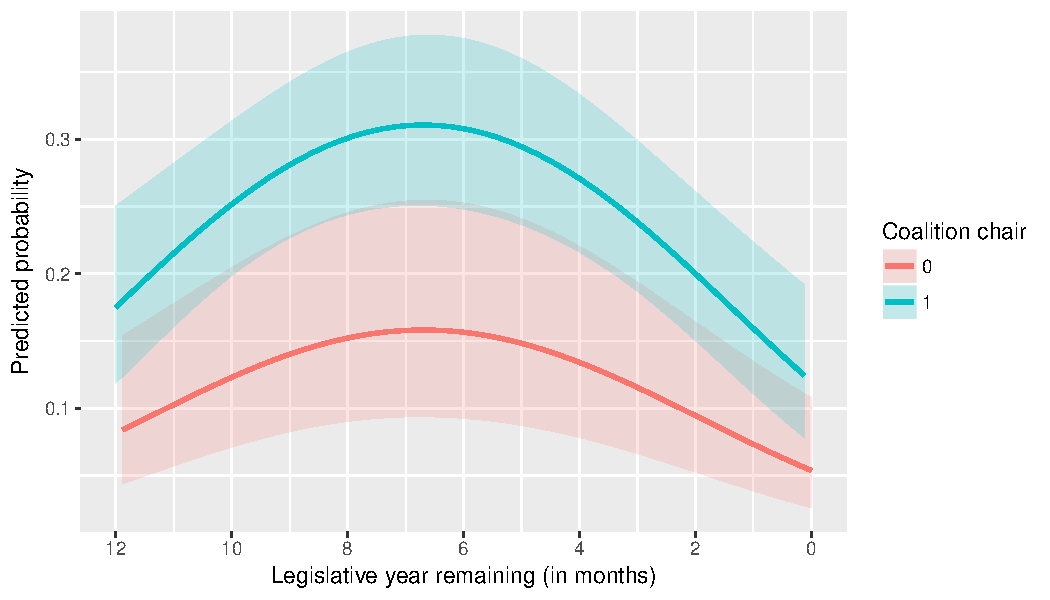
\includegraphics[width=.75\columnwidth]{../graphs/predictedPr.pdf}
\end{figure}

Finally, there are time trends in fast-track authority that simulations reveal neatly. Figure \ref{F:sims} portrays the predicted probability that a bill enters the fast-track throughout the legislative year. Regressors in model 3 are held constant to simulate a bill sent to the \emph{C\'amara} in the 2006--10 Legislature that was referred to a single committee, excluding \emph{Hacienda}. \emph{Presidential Approval} (insignificant across models) is set to the mean for President Bachelet's first term, coinciding in full with the 2006--10 Legislature. The inverted-U shape shows how fast-track probability, predicted at 0.17 for coalition-chaired committees at the start, and 0.08 for the rest, becomes much likelier in the first half of the legislative year. By the second quarter (June--August), the probability is at its peak, about 0.32 percent and 0.17, respectively. It then experiences a sharp drop, ending the austral Summer break at 0.13 for coalition-chaired committees, and 0.05 for others. And while 95-percent confidence bands overlap, they barely do so at the middle of the legislative year, lending confidence that we are picking up a signal and not just random noise. 

\section*{Discussion}\label{s:discussion}

This paper has argued that beyond the effect of urgency authority on the timing and deadlines for bill consideration, its procedural effects conceal a much more significant effect, by allowing presidents to shield desired policy from amendments on the floor. Furthermore, the president's decision not to use this tool is also important. An open rule means that bills can receive amendments on the floor that may move it closer to the president's preferences. This paper portrays urgency authority, found in seven Latin American constitutions, as equivalent to the fast-track authority that United States presidents enjoy periodically. Doing so shows how proposals that presidents qualify as urgent are considered under restrictive rules by the chamber's plenary: they must be voted up-or-down, without amendments.

While all seven constitutions remain silent about the procedural implications of urgency authority, and we have only looked for these restrictive procedures in statutes and chamber rules in the case of Chile, there are good reasons to expect that other countries have included similar provisions. After all, the rationale of the urgency authority is expediting the legislative process, and restrictive rules are a natural choice to speed urgent bills' consideration before an explicit deadline expires. 

The classification of constitutional urgency authority into the plenary arrest (Brazil), automatic adoption (Ecuador, Paraguay, Uruguay), and indeterminate (Chile, Colombia, Mexico) variants, which we presented in Section 2, naturally brings two pending issues to the fore. One is cross-national validation of the presence of restrictive procedures at the level of statutes or chamber rules---especially where urgency effects are seemingly indeterminate, as in Chile. The task ahead is to identify procedures that restrict the choices available to legislators, such as closed rules do in Chile. The other is the need to model the bargaining logic of plenary-arrest and automatic-adoption variants in search of similarities and differences with the urgency-as-fast-track. We expect these efforts to generalize our argument beyond Chile, our case study.

Game-theoretic treatment of urgency-as-fast-track authority shows that preference overlap between the president and the reporting committee is the mechanism driving the choice to put bills on the fast-track. The reverse also applies: bills referred to opposition-chaired committees, who might report them to the floor with fundamental changes, are less likely to be fast tracked. The president would prefer them to go to the floor with an open rule, especially if on the floor a (friendlier) majority can restore the original intent of the president and her party. Systematic analysis of proposals in the Chilean lower chamber in recent years yields evidence that, other things constant, bills reported by committees chaired by members of the president's coalition/party are about twice as likely to be fast-tracked than the rest. To the extent that parties and coalitions indicate preference overlap (as is accepted in Chile), the evidence supports our main theoretical result.

The paper's results and findings are of natural interest to students of comparative political institutions, especially those interested in legislative procedure and separation of powers. They also shed light on the field of American Politics. In a provocative book, \citet{howell.moe.Relic2016} make an argument in favor of giving U.S.\ presidents permanent fast-track authority not limited to trade agreements. In order to have a coherent and effective government, they argue in favor of constitutional reform to put the executive at the center of the legislative process: ``presidents should be granted enhanced agenda-setting powers to propose bills to Congress, which Congress should then be required to vote on without amendment, on a strictly majoritarian basis, within a fixed period of time'' \citep[][, 145]{howell.moe.Relic2016}. Failure to vote in due time would turn those bills into law. Equating urgency and fast-track authorities shows this to be the automatic adoption variant. Reform would therefore make U.S.\ presidents similar to those in Ecuador, Paraguay, and Uruguay in this respect. 

Our results also speak to students of executive decrees and unilateral policymaking more generally. As discussed at the start of the paper, urgency authority and decree authority may overlap, as in fact they do in Brazil, Chile, and Colombia. We have established that, while urgency authority increases the president's leverage over the legislative process, an agreement is needed between the president and her congressional allies without which this prerogative is rendered powerless. Congress retains authority to reject urgent proposals, and cannot therefore be made worse-off than the status quo. Executive decrees, on the other hand, imply an abdication of decision rights on the part of legislators to participate in the process, and force legislators to respond to the president's enacted decree instead once it has already altered the status quo.

Yet for this precise reason executive decrees are not a true alternative in certain cases \citep{palanza.2019}. \citet[][, 164]{figueiredo.limongi.2000} report that urgent bills in Brazil are quite rare since the provisional decree ``is a much more efficient way of speeding up and approving legislation.'' More research should be done to establish whether effectively the urgency prerogative is used, for instance, on issues that are excluded from executive decree authority in the Brazilian constitution. Previous findings indicate that reliance on decrees effectively diminishes when policy deals with these issues---although it does not disappear. It is undeniable that Chile, where executive decrees are seldom used (only two decrees have been enacted since 1990), resorts to urgency authority expansively. Future research, and hopefully comparative work, will help tackle this issue. 

Chilean legislative scholars will find interest in investigating a missing piece in our argument. To be clear, the research advanced in this paper sheds light on the factors that affect the likelihood of reliance on urgency authority, and we provide an argument explaining the mechanism that leads to this usage. But we do not provide verification that closed rules do in fact dispel amendments---a key and untested premise of our approach. Systematic contrasting of bills that presidents drafted in the period, the various amendments that were introduced, the committee reports, and the text ultimately adopted, would enable analysts to demonstrate whether or not urgencies in fact dodge amendments. This is a difficult but promising venue for future research. 

Last, we emphasize that our investigation contributes to the literature on restrictive procedures. To the general class of procedures as instruments of political control, we add the urgency authority. One difference sets fast-track mechanisms apart from standard closed rules. Standard restrictive rules give agenda power to legislators---it may be the plenary \citep{mcnollgast.1987}, standing committees \citep{weingast.1992}, the bicameral conference \citep{shepsle.weingast.1987}, or the majority party \citep{cox.mccubbins.1997}. Urgency puts the executive in control of protecting vulnerable legislative agreements. The unique role and function to determine whether or not a major bill will be considered in the U.S. House, and which amendments and motions will be allowed, is firmly in control of the legislative leadership, acting as sole gatekeepers to the plenary \citep{cox.2006}. As with France's \emph{vote bloqu\'e} \citep{huber.1996b}, fast-track authority lets the executive branch pull some of the gatekeeping levers, earning a priceless legislative prerogative worthy of further research.

%% \section*{Author contributions}

%% We describe contributions to the paper using a standard taxonomy \citep{allen2014credit}. E.\ Magar (EM) was lead author, having taken primary responsibility for methodology, computation, formal analysis, and data collection and curation. G.\ Sin (GS) was responsible for comparative constitutional research. V.\ Palanza (VP) was in charge of funding acquisition. EM prepared the original draft and revision for resubmission. VP lead text editing and review, with contributions from GS. All authors contributed equally to conceptualization and article framing. 

%\singlespacing

\section*{Acknowledgements}
The authors are grateful to Roberto Bustos, Alvaro Villarroel, and the staff of the Chilean Senate's Hacienda Committee, and especially to Sebasti\'an Soto Velasco for help understanding urgency authority; to Diputado Patricio Vallesp\'in for making the calls that scheduled interviews with key congressional personnel; to M\'onica Arretche, Ernesto Calvo, Jos\'e Antonio Cheibub, Federico Est\'evez, Adri\'an Lucardi, Michelle Taylor-Robinson, three anonymous reviewers, and participants at the 2017 annual meeting of the American Political Science Association in San Francisco, at the Evolution of Parliamentarism Workshop in Rome, and at the IV encuentro del Grupo de Estudios Legislativos de \textsc{alacip} in Mexico City for critiques and suggestions. Eric Magar received financial support from the Asociaci\'on Mexicana de Cultura \textsc{a.c.}\ and \textsc{conacyt}'s Sistema Nacional de Investigadores. Valeria Palanza received support from Proyecto Fondecyt No.\ 1140974. Gisela Sin received the support of the Office of the Vice Chancellor for Research and the Center for Latin American Studies, University of Illinois at Urbana-Champaign. The authors are responsible for mistakes and shortcomings in the study.

\listofendnotes

\bibliographystyle{apsr}

%\bibliography{../bib/magar}

\begin{thebibliography}{xx}

\harvarditem{Alem\'an \harvardand\ Tsebelis}{2016}{aleman-tsebelis-2016-book}
Alem\'an, Eduardo \harvardand\ George Tsebelis. 2016.
\newblock {\em Legislative Institutions and Lawmaking in Latin America}.
\newblock Oxford:  Oxford University Press.

\harvarditem{Alem\'an \harvardand\ Navia}{2009}{aleman.navia.UrgChi.2009}
Alem\'an, Eduardo \harvardand\ Patricio Navia. 2009.
\newblock ``Institutions and the Legislative Success of `Strong' Presidents: An
  Analysis of Government Bills in {Chile}.'' {\em Journal of Legislative
  Studies} 15(4):401--19.

\harvarditem{Alem\'an \harvardand\
  Saiegh}{2007}{aleman.saiegh.coalUnityChile.2007}
Alem\'an, Eduardo \harvardand\ Sebasti\'an~M. Saiegh. 2007.
\newblock ``Legislative Preferences, Political Parties, and Coalition Unity in
  Chile.'' {\em Comparative Politics} 39(April):253--72.

\harvarditem[Amorim~Neto, Cox \harvardand\ McCubbins]{Amorim~Neto, Cox
  \harvardand\ McCubbins}{2003}{amorim.cox.mccubbins.2003}
Amorim~Neto, Oct\'avio, Gary~W. Cox \harvardand\ Mathew~D. McCubbins. 2003.
\newblock ``Agenda Power in Brazil's C\^amara dos Deputados, 1989--98.'' {\em
  World Politics} 55:550--78.

\harvarditem{Aninat}{2006}{aninat.exagCoop2006}
Aninat, Crist\'obal. 2006.
\newblock ``Balance de poderes legislativos en Chile. ¿Presidencialismo
  exagerado o base de un sistema pol\'itico cooperativo?'' {\em Revista de
  Ciencia Pol\'itica} 47(1):127--48.

\harvarditem[Bates et~al.]{Bates, Maechler, Bolker \harvardand\
  Walker}{2015}{lme4.2015}
Bates, Douglas, Martin Maechler, Benjamin~M. Bolker \harvardand\ Steven Walker.
  2015.
\newblock ``Fitting Linear Mixed-Effects Models using {lme4}.''.
\newblock ArXiv e-print; in press, \emph{Journal of Statistical Software}.
\newline\harvardurl{http://arxiv.org/abs/1406.5823}

\harvarditem{Berr\'ios \harvardand\
  Gamboa}{2006}{berrios.gamboa.fiscChile.2006}
Berr\'ios, Fabiola \harvardand\ Ricardo Gamboa. 2006.
\newblock ``El {Congreso Nacional} chileno y el ejercicio de sus funciones
  legislativa y fiscalizadora (1990--2006).'' {\em Pol\'itica} 47(1):99--125.

\harvarditem{Bond \harvardand\ Fleisher}{1990}{bond.fleisher.1990}
Bond, Jon~R. \harvardand\ Richard Fleisher. 1990.
\newblock {\em The President in the Legislative Arena}.
\newblock Chicago:  Chicago University Press.

\harvarditem{Calvo}{2014}{calvo.2014argBook}
Calvo, Ernesto. 2014.
\newblock {\em Legislator success in fragmented congresses in {A}rgentina:
  Plurality cartels, minority presidents, and lawmaking}.
\newblock New York:  Cambridge University Press.

\harvarditem{Carey}{2002}{carey.2002}
Carey, John~M. 2002.
\newblock Parties, Coalitions, and the {Chilean} Congress in the 1990s.  In
  {\em Legislative Politics in Latin America}, ed. Scott Morgenstern
  \harvardand\ Benito Nacif.
\newblock New York:  Cambridge University Press pp.~222--53.

\harvarditem{Carey \harvardand\ Shugart}{1998}{carey.shugart.1998}
Carey, John~M. \harvardand\ Matthew~S. Shugart, eds. 1998.
\newblock {\em Executive Decree Authority}.
\newblock New York:  Cambridge University Press.

\harvarditem{Carroll \harvardand\ Pach\'on}{2016}{carroll-pachon.2016}
Carroll, Royce \harvardand\ M\'onica Pach\'on. 2016.
\newblock The Unrealized Potential of Presidential Coalitions in Colombia.  In
  {\em Legislative Institutions and Lawmaking in Latin America}, ed. Eduardo
  Alem\'an \harvardand\ George Tsebelis.
\newblock Oxford:  Oxford University Press.

\harvarditem{Chasquetti}{2016}{chasquetti.2016}
Chasquetti, Daniel. 2016.
\newblock Agenda setting and Lawmaking in Uruguay.  In {\em Legislative
  Institutions and Lawmaking in Latin America}, ed. Eduardo Alem\'an
  \harvardand\ George Tsebelis.
\newblock Oxford:  Oxford University Press.

\harvarditem{Cox}{2006}{cox.2006}
Cox, Gary~W. 2006.
\newblock The Organization of Democratic Legislatures.  In {\em The Oxford
  Handbook of Political Economy}, ed. Barry~R. Weingast \harvardand\ Donald~A.
  Wittman.
\newblock New York:  Oxford University Press pp.~141--61.

\harvarditem{Cox \harvardand\ McCubbins}{1993}{cox.mccubbins.1993}
Cox, Gary~W. \harvardand\ Mathew~D. McCubbins. 1993.
\newblock {\em Legislative {L}eviathan: Party Government in the {H}ouse}.
\newblock Berkeley:  University of California Press.

\harvarditem{Cox \harvardand\ McCubbins}{1997}{cox.mccubbins.1997}
Cox, Gary~W. \harvardand\ Mathew~D. McCubbins. 1997.
\newblock ``Toward a theory of legislative rules changes: Assessing {S}chickler
  and {R}ich's evidence.'' {\em American Journal of Political Science}
  41(4):1376--86.

\harvarditem{Cox \harvardand\ McCubbins}{2005}{cox.mccubbins.2005}
Cox, Gary~W. \harvardand\ Mathew~D. McCubbins. 2005.
\newblock {\em Setting the Agenda: Responsible Party Government in the {US}
  {H}ouse of {R}epresentatives}.
\newblock New York:  Cambridge University Press.

\harvarditem{Danesi}{2010}{danesi.2010}
Danesi, Silvina~L. 2010.
\newblock The Institutional Choices of Politicians: How and Why Legislators
  Shape Lower Chambers PhD thesis Universit\'e de Montr\'eal.

\harvarditem{Den~Hartog}{2004}{denhartog.2004phd}
Den~Hartog, Christopher~F. 2004.
\newblock Limited Party Government and the Majority Party Revolution in the
  Nineteenth-Century {H}ouse PhD thesis UCSD.

\harvarditem{Destler}{1991}{destler-1991}
Destler, I.M. 1991.
\newblock U.S. Trade Policy-making in the Eighties.  In {\em Politics and
  Economics in the Eighties}, ed. Alberto Alesina \harvardand\ Geoffrey
  Carliner.
\newblock Chicago, IL:  University of Chicago Press.

\harvarditem{Destler}{1992}{destler-1992}
Destler, I.M. 1992.
\newblock {\em American Trade Politics}.
\newblock Washington, D.C.:  Institute for International Economics.

\harvarditem{Dion \harvardand\ Huber}{1996}{dion.huber.1996}
Dion, Douglas \harvardand\ John~D. Huber. 1996.
\newblock ``Procedural Choice and the {H}ouse Committee on Rules.'' {\em The
  Journal of Politics} 58(1):25--53.

\harvarditem{D{\"o}ring}{2003}{doring.restrictiveRules.2003}
D{\"o}ring, Herbert. 2003.
\newblock ``Party discipline and government imposition of restrictive rules.''
  {\em Journal of Legislative Studies} 9(4):147--63.

\harvarditem{Fergusson}{2015}{crs-2015-tpa}
Fergusson, Ian~F. 2015.
\newblock ``Trade Promotion Authority (TPA) and the Role of Congress in Trade
  Policy.'' Congressional Research Service RL33743 \url{www.crs.gov}.

\harvarditem{Figueiredo \harvardand\ Limongi}{2000}{figueiredo.limongi.2000}
Figueiredo, Argelina~Cheibub \harvardand\ Fernando Limongi. 2000.
\newblock ``Presidential Power, Legislative Organization, and Party Behavior in
  Brazil.'' {\em Comparative Politics} 32(1):151--70.

\harvarditem{Garc\'ia~Montero}{2009}{garcia.montero.presidentes.2009}
Garc\'ia~Montero, Mercedes. 2009.
\newblock {\em Presidentes y parlamentos: ?`qui\'en controla la actividad
  legislativa en {A}m\'erica {L}atina?}
\newblock Vol. Colecci\'on Monograf\'ias 269 Madrid:  Centro de Investigaciones
  Sociol\'ogicas.

\harvarditem{Gelman \harvardand\ Hill}{2007}{gelman.hill.2007}
Gelman, Andrew \harvardand\ Jennifer Hill. 2007.
\newblock {\em Data Analysis Using Regression and Multilevel/Hierarchical
  Models}.
\newblock Cambridge University Press.

\harvarditem{Gerber}{1996}{gerber.1996}
Gerber, Elisabeth~R. 1996.
\newblock ``Legislative Responses to the Threat of Popular Initiatives.'' {\em
  American Journal of Political Science} 40(1):99--128.

\harvarditem{Goldstein}{1988}{goldstein-1988}
Goldstein, Judith. 1988.
\newblock ``Ideas, Institutions and American Trade Policy.'' {\em International
  Organization} 42(Winter):179--217.

\harvarditem{Haggard}{1988}{haggard-1988}
Haggard, Stephan. 1988.
\newblock ``The Institutional Foundations of Hegemony.'' {\em International
  Organization} 42(Winter):91--119.

\harvarditem{Hamilton}{1961}{hamilton70.1788}
Hamilton, Alexander. 1961.
\newblock The Federalist \textsc{lxx}.  In {\em The Federalist Papers:
  Hamilton, Madison, Jay}, ed. Clinton Rossiter.
\newblock New York:  Penguin.

\harvarditem{Heller}{2001}{heller.2001}
Heller, William~B. 2001.
\newblock ``Making Policy Stick: Why the Government Gets What It Wants in
  Multiparty Parliaments.'' {\em American Journal of Political Science}
  45(4):780--98.

\harvarditem{Hiroi \harvardand\ Renn\'o}{2016}{hiroi-renno-2016}
Hiroi, Taeko \harvardand\ Lucio Renn\'o. 2016.
\newblock Agenda Setting and Gridlock in a Multiparty Coalitional Presidential
  System: The Case of Brazil.  In {\em Legislative Institutions and Lawmaking
  in Latin America}, ed. Eduardo Alem\'an \harvardand\ George Tsebelis.
\newblock Oxford:  Oxford University Press.

\harvarditem{Howell \harvardand\ Moe}{2016}{howell.moe.Relic2016}
Howell, William~G. \harvardand\ Terry~M. Moe. 2016.
\newblock {\em Relic: How our Constitution Undermines Effective
  Government---and Why We Need a More Powerful Presidency}.
\newblock New York:  Basic Books.

\harvarditem{Huber}{1996}{huber.1996b}
Huber, John~D. 1996.
\newblock {\em Rationalizing Parliament: Legislative Institutions and Party
  Politics in France}.
\newblock New York:  Cambridge University Press.

\harvarditem{Kiewiet \harvardand\ McCubbins}{1991}{kiewiet.mccubbins.1991}
Kiewiet, D.~Roderick \harvardand\ Mathew~D. McCubbins. 1991.
\newblock {\em The Logic of Delegation: Congressional Parties and the
  Appropriations Process}.
\newblock Chicago:  University of Chicago Press.

\harvarditem{Krehbiel}{1997}{krehbielRestrictiveRules1997}
Krehbiel, Keith. 1997.
\newblock ``Restrictive Rules Reconsidered.'' {\em American Journal of
  Political Science} 41(3):919--44.

\harvarditem{Lohmann \harvardand\ O'Halloran}{1994}{lohmann-ohalloran.1994}
Lohmann, Susanne \harvardand\ Sharyn O'Halloran. 1994.
\newblock ``Divided government and U.S. trade policy: theory and evidence.''
  {\em International Organization} 48(4):595--632.

\harvarditem{Magar}{2007}{magar.stunts.ssrn.2007}
Magar, Eric. 2007.
\newblock ``Executive Vetoes as Electoral Stunts: A Model with Testable
  Predictions.'' {\em SSRN eLibrary} .
\newline\harvardurl{http://dx.doi.org/10.2139/ssrn.1486804}

\harvarditem{Magar}{2014}{magar.2014-refConst}
Magar, Eric. 2014.
\newblock Los contados cambios al equilibrio de poderes.  In {\em Reformar sin
  mayor\'ias: La din\'amica del cambio constitucional en {M}\'exico,
  1997--2012}, ed. Mar\'ia~Amparo Casar \harvardand\ Ignacio Marv\'an~Laborde.
\newblock Mexico City:  Taurus pp.~259--94.

\harvarditem{Margolis}{1986}{margolis-1986}
Margolis, Lawrence. 1986.
\newblock {\em Executive Agreements and Presidential Power in Foreign Policy}.
\newblock New York:  Preager.

\harvarditem[McCubbins, Noll \harvardand\ Weingast]{McCubbins, Noll
  \harvardand\ Weingast}{1987}{mcnollgast.1987}
McCubbins, Mathew~D., Roger~G. Noll \harvardand\ Barry~R. Weingast. 1987.
\newblock ``Administrative Procedures as Instruments of Political Control.''
  {\em Journal of Law, Economics, \& Organization} 3(1):243--77.

\harvarditem{Morgenstern \harvardand\ Nacif}{2002}{morgenstern.nacif.2002}
Morgenstern, Scott \harvardand\ Benito Nacif. 2002.
\newblock {\em Legislative Politics in Latin America}.
\newblock New York:  Cambridge University Press.

\harvarditem[Morgenstern, Polga-Hecimovich \harvardand\
  Shair-Rosenfeld]{Morgenstern, Polga-Hecimovich \harvardand\
  Shair-Rosenfeld}{2013}{morgenstern-polga-shair.2013}
Morgenstern, Scott, Polga-Hecimovich \harvardand\ Sarah Shair-Rosenfeld. 2013.
\newblock ``Tall, Grande, or Venti: Presidential Powers in the United States
  and Latin America.'' {\em Journal of Politics in Latin America} 2(1):37--70.

\harvarditem{Nolte}{2003}{nolte.2003}
Nolte, Detlef. 2003.
\newblock ``El Congreso chileno y su aporte a la consolidaci\'on democr\'atica
  en perspectiva comparada.'' {\em Revista de Ciencia Pol\'itica} 23(2):43--67.

\harvarditem{Oleszek}{2001}{oleszek.2001}
Oleszek, Walter~J. 2001.
\newblock {\em Congressional Procedures and the Policy Process}.
\newblock 5$^{th}$ ed. Washington DC:  Congressional Quarterly Press.

\harvarditem{Palanza}{2019}{palanza.2019}
Palanza, Valeria. 2019.
\newblock {\em Checking Presidential Power: Executive Decrees and the
  Legislative Process in New Democracies}.
\newblock New York:  Cambridge University Press.

\harvarditem{Romer \harvardand\ Rosenthal}{1978}{romer.rosenthal.1978}
Romer, Thomas \harvardand\ Howard Rosenthal. 1978.
\newblock ``Political resource allocation, controlled agendas, and the status
  quo.'' {\em Public Choice} 33:27--44.

\harvarditem{Schickler \harvardand\ Rich}{1997}{schickler.richRules1997}
Schickler, Eric \harvardand\ Andrew Rich. 1997.
\newblock ``Controlling the Floor: Procedural Coalitions in the {H}ouse.'' {\em
  American Journal of Political Science} 41(4):1340--75.

\harvarditem{Shepsle}{1979}{shepsle.1979}
Shepsle, Kenneth~A. 1979.
\newblock ``Institutional Arrangements and Equilibrium in Multidimensional
  Voting Models.'' {\em American Journal of Political Science} 23(1):27--59.

\harvarditem{Shepsle \harvardand\ Weingast}{1987}{shepsle.weingast.1987}
Shepsle, Kenneth~A. \harvardand\ Barry~R. Weingast. 1987.
\newblock ``The Institutional Foundations of Committee Power.'' {\em American
  Political Science Review} 81(1):85--104.

\harvarditem{Siavelis}{2002}{siavelis.2002}
Siavelis, Peter. 2002.
\newblock Exaggerated Presidentialism and Moderate Presidents:
  Executive-Legislative Relations in {Chile}.  In {\em Legislative Politics in
  Latin America}, ed. Scott Morgenstern \harvardand\ Benito Nacif.
\newblock New York:  Cambridge University Press.

\harvarditem{Sin}{2014}{sin.2014}
Sin, Gisela. 2014.
\newblock {\em Separation of Powers and Legislative Organization: The
  President, the Senate, and Political Parties in the Making of House Rules}.
\newblock New York, NY:  Cambridge University Press.

\harvarditem{Soto~Velasco}{2015}{sotoCongChile2015}
Soto~Velasco, Sebasti\'an. 2015.
\newblock {\em Congreso Nacional y Proceso Legislativo: Teor\'ia y Pr\'actica}.
\newblock Santiago:  Thomson Reuters.

\harvarditem{Weingast}{1992}{weingast.1992}
Weingast, Barry~R. 1992.
\newblock Fighting Fire with Fire: Amending Activity and Institutional Change
  in the Postreform Congress.  In {\em The Postreform Congress}, ed. Roger~H.
  Davidson.
\newblock St.\ Martin's Press.

\end{thebibliography}


\end{document}

